\documentclass[12pt]{article}
\usepackage[utf8]{inputenc}
\usepackage{hyperref}
\usepackage{tikz}
\usepackage{caption}
\usepackage{amsmath}
\usepackage[margin=1in]{geometry}
\usepackage{graphicx}

\title{}
\author{Shaan Fulton}
\date{\today}

\begin{document}

\maketitle

\section*{Search Problems}

Many problems can be understood as search problems. A search problem is any problem which involves a:

\begin{itemize}
	\item Set of possible states
	\item A start state
	\item A goal state
	\item A successor function (a function which returns what states can be achieved from a given state)
\end{itemize}

In other words, it's a problem where we must determine a set of actions (that fall within our successor function) to achieve our goal state from our start state.

\section*{Pathfinding as a Search Problem}

\subsection*{1. Set of Possible States}

Each state is a position on a grid. Here is the full set of states for a 3x3 grid:

\begin{center}
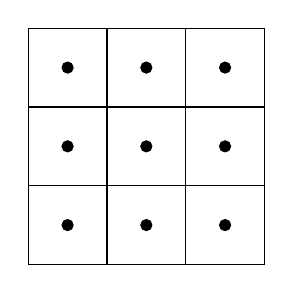
\begin{tikzpicture}
    \foreach \x in {0,1,2} {
        \foreach \y in {0,1,2} {
            \draw (\x, \y) rectangle ++(1,1);
            \filldraw[black] (\x+0.5, \y+0.5) circle (2pt);
        }
    }
\end{tikzpicture}
\end{center}

This represents 9 possible states (positions), arranged in a 3x3 grid.

\subsection*{2. Start State}

\begin{center}
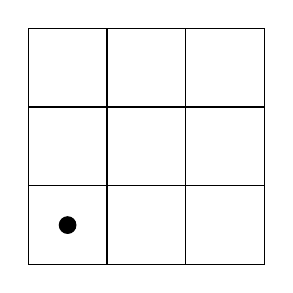
\begin{tikzpicture}
    \foreach \x in {0,1,2} {
        \foreach \y in {0,1,2} {
            \draw (\x, \y) rectangle ++(1,1);
        }
    }
    % Character at (0,0)
    \filldraw[black] (0.5, 0.5) circle (3pt);
\end{tikzpicture}
\captionof{figure}{Start state: character begins in the bottom-left corner}
\end{center}

\subsection*{3. Goal State}

\begin{center}
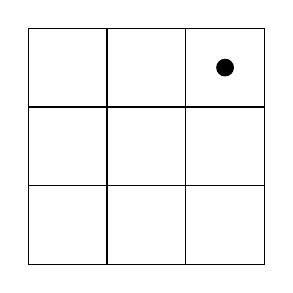
\begin{tikzpicture}
    \foreach \x in {0,1,2} {
        \foreach \y in {0,1,2} {
            \draw (\x, \y) rectangle ++(1,1);
        }
    }
    % Character at (2,2)
    \filldraw[black] (2.5, 2.5) circle (3pt);
\end{tikzpicture}
\captionof{figure}{Goal state: character must reach the top-right corner}
\end{center}

\subsection*{4. Successor Function}

From any given position, the character can move one square up, down, left, or right (if within bounds). For example, from the center of the grid:

\begin{center}
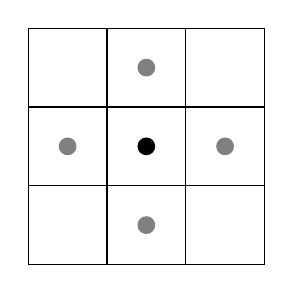
\begin{tikzpicture}
    % Draw the grid
    \foreach \x in {0,1,2} {
        \foreach \y in {0,1,2} {
            \draw (\x, \y) rectangle ++(1,1);
        }
    }
    % Main character at center
    \filldraw[black] (1.5, 1.5) circle (3pt);
    % Gray potential successors
    \filldraw[gray] (0.5, 1.5) circle (3pt); % left
    \filldraw[gray] (2.5, 1.5) circle (3pt); % right
    \filldraw[gray] (1.5, 0.5) circle (3pt); % down
    \filldraw[gray] (1.5, 2.5) circle (3pt); % up
\end{tikzpicture}
\end{center}

From the center, the successor function returns:
\begin{itemize}
    \item Move up: (1,2)
    \item Move down: (1,0)
    \item Move left: (0,1)
    \item Move right: (2,1)
\end{itemize}

\bigskip

Thus, the problem of pathfinding — determining how to move from the start state to the goal state — is clearly a search problem. However, search problems extend beyond pathfinding. The Tower of Hanoi is a famous example.

\begin{figure}[h]
  \centering
  \includegraphics[width=0.5\textwidth]{general-search-hanoi.jpg}
  \caption{The Tower of Hanoi, Solved}
  \label{fig:tower}
\end{figure}

Excellent overview \href{https://youtu.be/Mlwrx7hbKPs?t=3913}{found here.}

\end{document}

